\documentclass[11pt]{article}
\usepackage{upquote}
\usepackage{minted}
\fvset{frame=single}

\usepackage[colorlinks=true]{hyperref}
\usepackage[margin=1in]{geometry}
\usepackage{ifthen}
\usepackage{fancyvrb}

\usepackage{listings}
\usepackage{color}

\definecolor{dkgreen}{rgb}{0,0.6,0}
\definecolor{gray}{rgb}{0.5,0.5,0.5}
\definecolor{mauve}{rgb}{0.58,0,0.82}

\lstset{frame=tb,
  language=Java,
  aboveskip=3mm,
  belowskip=3mm,
  showstringspaces=false,
  columns=flexible,
  basicstyle={\small\ttfamily},
  numbers=none,
  numberstyle=\tiny\color{gray},
  keywordstyle=\color{blue},
  commentstyle=\color{dkgreen},
  stringstyle=\color{mauve},
  breaklines=true,
  breakatwhitespace=true,
  tabsize=3
}

\usepackage{graphicx}
\usepackage{float}

\usepackage{amsmath}
\usepackage{amsfonts}
\usepackage{mathtools}

\usepackage{multirow}
\usepackage{enumitem}

\usepackage{comment}
\usepackage[usenames,dvipsnames,svgnames,table,hyperref]{xcolor}

\newcommand{\vect}[1]{\boldsymbol{#1}}
\newcommand{\matr}[1]{\boldsymbol{#1}}
\DeclareMathOperator*{\argmin}{arg\,min}
\DeclareMathOperator*{\argmax}{arg\,max}
\newcommand{\sol}[1]{{\bf{\color{magenta}{{Solution:}}}}}

\parfillskip=3em plus1fil

\title{CM146, Winter 2023 \\ Problem Set 4: Boosting, Unsupervised learning}
\begin{document}

\author{}
\date{}
\vspace{0in}
\maketitle
\vspace{-0.75in}

\section{Implementation: Clustering and PCA}


\subsection{PCA}
\subsubsection{(a) Visualization}
\sol x
\begin{minted}{python}

    X, y = get_lfw_data()
    show_image(X[0])
    show_image(X[11])
    show_image(X[42])
    show_image(np.mean(X, axis=0))
        
\end{minted}

\begin{center}
    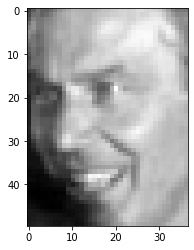
\includegraphics[scale=0.6]{1a-1.png}
\end{center}

\begin{center}
    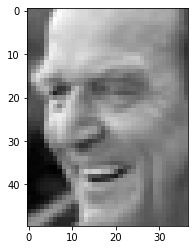
\includegraphics[scale=0.6]{1a-2.png}
\end{center}

\begin{center}
    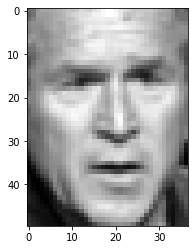
\includegraphics[scale=0.6]{1a-3.png}
\end{center}

The typical face, as shown below, appears quite ordinary since it features two dark shapes for eyes, some lines in the center for a nose, and a dark strip in the bottom half for a mouth. Since it represents an average, the face is positioned in the center of the picture, with the eyes, nose, and mouth roughly where they would be expected to be if you were looking at someone face-to-face.

\begin{center}
    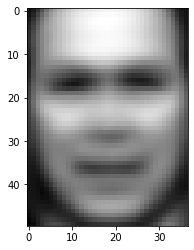
\includegraphics[scale=0.6]{1a-4.png}
\end{center}

\subsubsection{(b) Twelve Eigenfaces}
\sol x 
\begin{minted}{python}

    U, mu = util.PCA(X)
    plot_gallery([vec_to_image(U[:,i]) for i in range(12)])
        
\end{minted}

Out of the 12 images displayed below, it appears that each one differs from the others in some noticeable aspect: either the lighting is exceedingly bright or dark, or the face is either highly defined or not well defined. Furthermore, each face has a distinct appearance. These particular images were probably chosen because they represent the most distinctive and diverse eigenfaces. Since PCA was employed, we can understand it as though we will categorize the remaining images as containing features or components derived from these 12 faces.

\begin{center}
    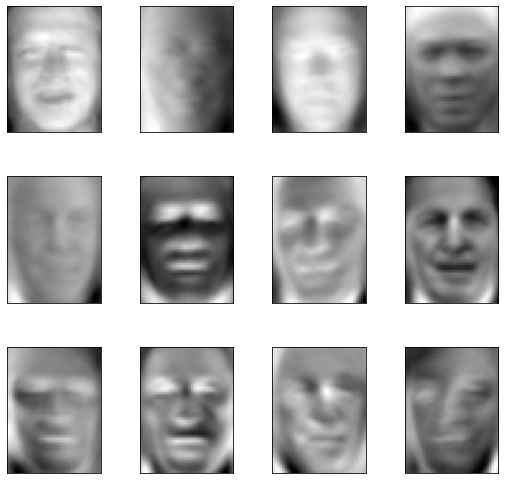
\includegraphics[scale=0.6]{1b.png}
\end{center}

\subsubsection{(c) Reconstruction under different number of components}
\sol x
\begin{minted}{python}

    l_values = [1, 10, 50, 100, 500, 1288]

    for l_value in l_values:
        Z, UI = apply_PCA_from_Eig(X, U, l_value, mu)
        X_rec = reconstruct_from_PCA(Z, UI, mu)
        title = f"Reconstructed for l = {l_value}"
        plot_gallery(X_rec, title=title)
        
\end{minted}

The pictures displayed below illustrate that as the value of "l" increases, the images become more distinct, clear, and detailed, retaining more information from the original image. This correlation makes sense because "l" denotes the number of components of the original image that we keep. The images with "l" equal to 1 look quite similar to each other and to the generic image (as seen in part (a)), as only the most significant component is retained. However, the images with "l" equal to 500 and 1288 are more detailed and can be more confidently attributed to a particular person. Interestingly, there was little difference between the images with "l" equal to 500 and 1288, suggesting that beyond "l" equal to 500, there may be diminishing returns. Therefore, for facial recognition purposes, an extremely low value of "l" is not useful since all images will appear the same, but a value of "l" that is excessively high, such as 1288, is also not helpful since it does not provide much additional clarity and may worsen performance by retaining too many principal components.

For l = 1:
\begin{center}
    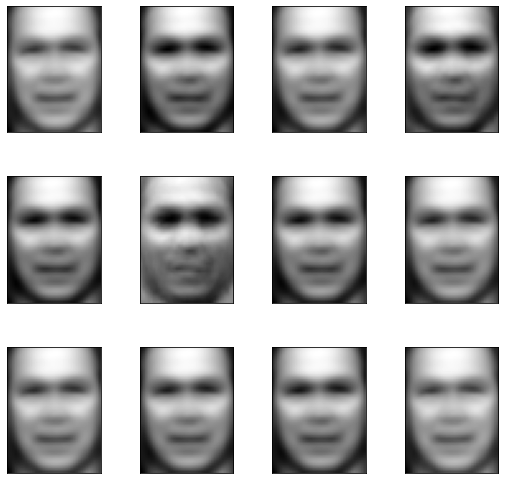
\includegraphics[scale=0.6]{1c-1.png}
\end{center}

For l = 10:
\begin{center}
    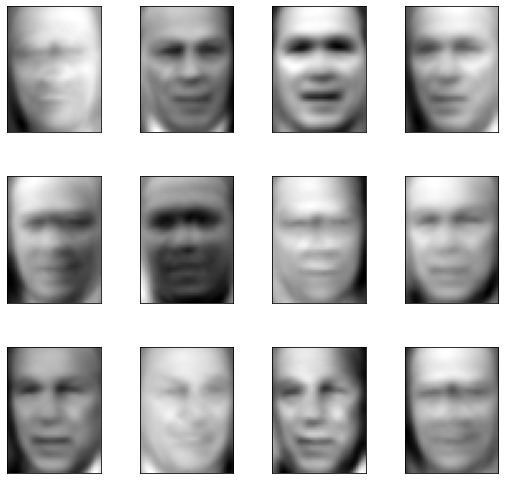
\includegraphics[scale=0.6]{1c-2.png}
\end{center}

For l = 50:
\begin{center}
    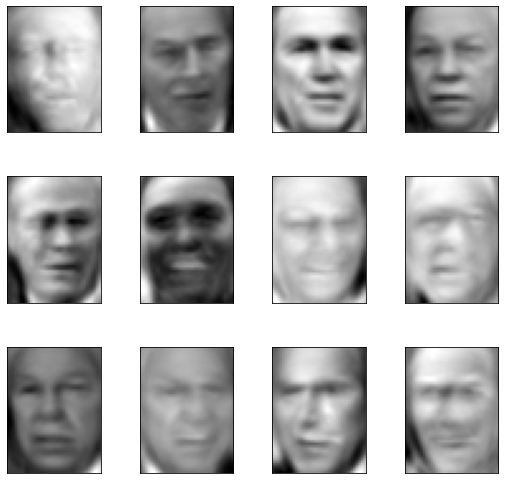
\includegraphics[scale=0.6]{1c-3.png}
\end{center}

For l = 100:
\begin{center}
    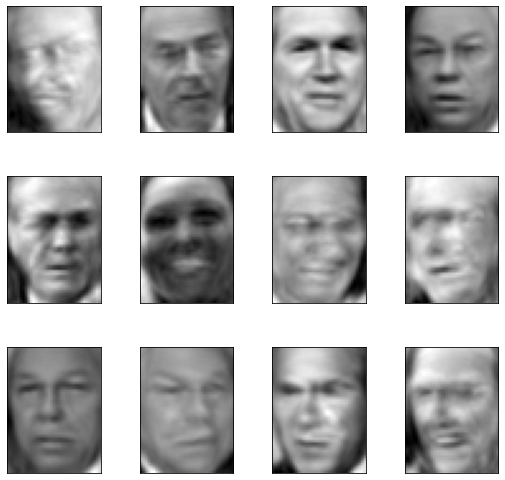
\includegraphics[scale=0.6]{1c-4.png}
\end{center}

For l = 500:
\begin{center}
    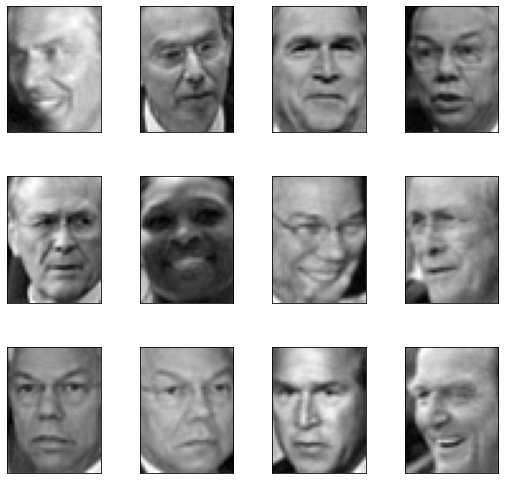
\includegraphics[scale=0.6]{1c-5.png}
\end{center}

For l = 1288:
\begin{center}
    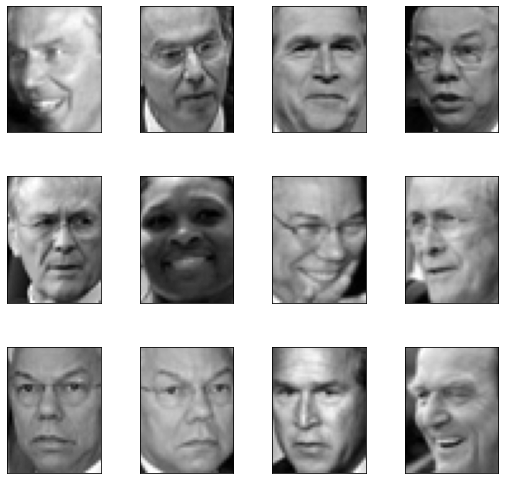
\includegraphics[scale=0.6]{1c-6.png}
\end{center}

\subsection{K-Means and K-Medoids}
\subsubsection{(a) Alternative optimization scheme}
\sol x Optimizing $\mu$, $c$, and $k$ without keeping $k$ constant would not be a good strategy, as the optimal solution would be achieved by setting $k$ equal to $n$. However, this would not be a meaningful clustering, as each point would become the center of its own cluster, yielding no new information. In this $k = n$ scenario, every point would be assigned to a cluster with a center at its own location, resulting in a cost of 0. $\boldsymbol{\mu}_i$ would simply be $\mathbf{x}_i$, and $c$ would be equal to $i$.

\subsubsection{(b) Implementation of Cluster and ClusterSet class}
\sol x
\begin{minted}{python}

    def centroid(self):
        label_count = {}
        avg_attributes = np.mean(np.array([p.attrs for p in self.points]), axis=0)

        for point in self.points:
            if point.label not in label_count:
                label_count[point.label] = 0
            label_count[point.label] += 1

        label_max = max(label_count, key=label_count.get)
        centroid = Point('centroid', label_max, avg_attributes)

        return centroid
        
\end{minted}

\begin{minted}{python}

    def medoid(self):
        distances = np.zeros((len(self.points), len(self.points)))

        for i in range(len(self.points)):
            for j in range(len(self.points)):
                if i != j:
                    distances[i][j] = self.points[i].distance(self.points[j])
                
        distance_sums = np.sum(distances, axis=0)
        point_num = np.argmin(distance_sums)
        return self.points[point_num]     
        
\end{minted}

\begin{minted}{python}

    def centroids(self):
        centroids = [cluster.centroid() for cluster in self.members]
        return centroids
        
\end{minted}

\begin{minted}{python}

    def medoids(self):
        medoids = [cluster.medoid() for cluster in self.members]
        return medoids
        
\end{minted}

\subsubsection{(c) Implementation of random\_init and kMeans}
\sol{} 
\begin{minted}{python}

    def random_init(points, k):
        return np.random.choice(points, k, replace=False)
        
\end{minted}

\begin{minted}{python}
    
    def kMeans(points, k, init='random', plot=False):
        k_clusters = ClusterSet()
        k_clusters_old = k_clusters
        k_clusters_new = ClusterSet()
        cluster_points = {}
        i = 1
    
        if init == 'random':
            initial_pts = random_init(points, k)
        elif init == 'cheat':
            initial_pts = cheat_init(points)
    
        curr_centroids = initial_pts
    
        while True:
            for point in points:
                min_dist = float('inf')
                best_centroid = None
                for centroid in curr_centroids:
                    distance = point.distance(centroid)
                    if distance < min_dist:
                        min_dist = distance
                        best_centroid = centroid
                if best_centroid not in cluster_points:
                    cluster_points[best_centroid] = []
                cluster_points[best_centroid].append(point)
    
            for key in cluster_points:
                k_clusters_new.add(Cluster(cluster_points[key]))
            cluster_points.clear()
    
            plot_title = f"K-means Iteration #{i}"
            if init == 'cheat':
                plot_title += ' - Cheat Init'
            if plot:
                plot_clusters(k_clusters_new, title=plot_title, average=ClusterSet.centroids)
    
            if k_clusters_new.equivalent(k_clusters_old):
                break
    
            k_clusters_old = k_clusters_new
            k_clusters_new = ClusterSet()
            i += 1
            curr_centroids = k_clusters_old.centroids()
    
        return k_clusters_old
        
\end{minted}
\subsubsection{(d) Behavior of kMeans}
\sol x The cluster set converged to a value after 3 iterations: the 4th iteration has the exact same values as the 3rd.

\begin{center}
    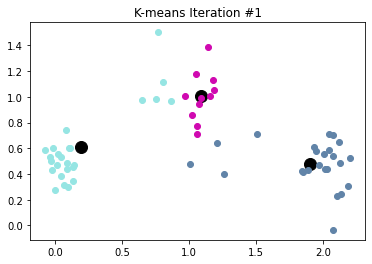
\includegraphics[scale=0.6]{2d-1.png}
\end{center}

\begin{center}
    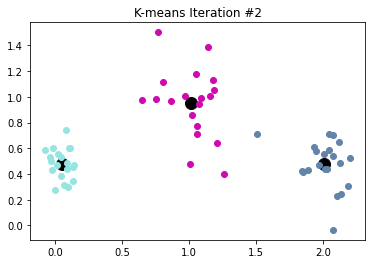
\includegraphics[scale=0.6]{2d-2.png}
\end{center}

\begin{center}
    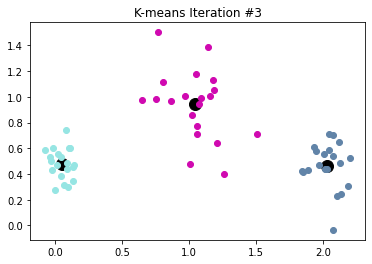
\includegraphics[scale=0.6]{2d-3.png}
\end{center}

\begin{center}
    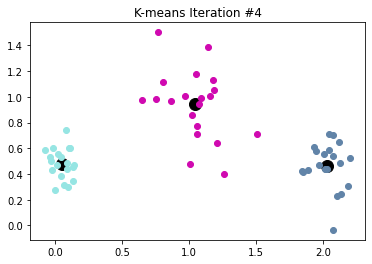
\includegraphics[scale=0.6]{2d-4.png}
\end{center}

\subsubsection{(e) Implementation and behavior of kMedoids}
\sol x Similar to part (d), the cluster set converged to a value after 3 iterations: the 4th iteration has the exact same values as the 3rd.

\begin{minted}{python}

    def kMedoids(points, k, init='random', plot=False):
        k_clusters = ClusterSet()
        k_clusters_old = k_clusters
        k_clusters_new = ClusterSet()
        cluster_points = {}
        i = 1
        if init == 'random':
            initial_pts = random_init(points, k)
        elif init == 'cheat':
            initial_pts = cheat_init(points)
        
        curr_medoids = initial_pts    
        while True:
            for point in points:
                min_dist = 100000
                best_medoid = None
                for medoid in curr_medoids:
                    distance = point.distance(medoid)
                    if distance<min_dist:
                        min_dist = distance
                        best_medoid = medoid
                if best_medoid not in cluster_points:
                    cluster_points[best_medoid] = []
                cluster_points[best_medoid].append(point)
            
            for key in cluster_points.keys(): 
                k_clusters_new.add(Cluster(cluster_points[key]))
            cluster_points.clear()
            plot_title = f"K-medoids Iteration #{i}"
            if init == 'cheat':
                plot_title += ' - Cheat Init'
            if plot:
                plot_clusters(k_clusters_new, title = plot_title, average=ClusterSet.medoids)
            if k_clusters_new.equivalent(k_clusters_old):
                break
            k_clusters_old = k_clusters_new
            k_clusters_new = ClusterSet()
            i = i+1
            curr_medoids = k_clusters_old.medoids()
    
        return k_clusters_old
    
\end{minted}

\begin{center}
    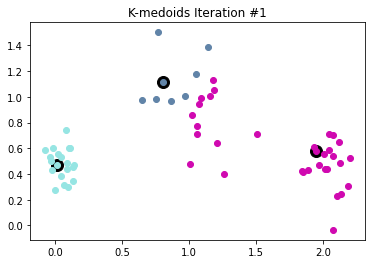
\includegraphics[scale=0.6]{2e-1.png}
\end{center}

\begin{center}
    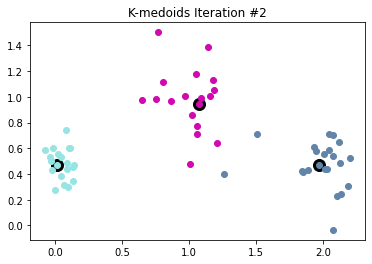
\includegraphics[scale=0.6]{2e-2.png}
\end{center}

\begin{center}
    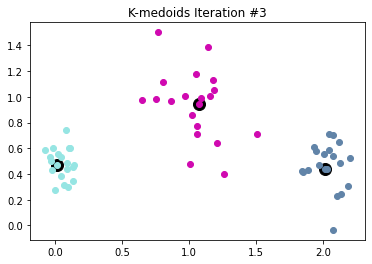
\includegraphics[scale=0.6]{2e-3.png}
\end{center}

\begin{center}
    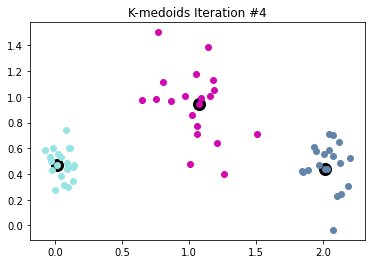
\includegraphics[scale=0.6]{2e-4.png}
\end{center}

\subsubsection{(f) Implementation and behavior of cheat\_init}
\sol x
\begin{minted}{python}

def cheat_init(points):
        initial_points = []
        cluster_labels = {}
        for point in points:
            if point.label not in cluster_labels:
                cluster_labels[point.label] = []
            cluster_labels[point.label].append(point)
        
        for key in cluster_labels.keys():
            cluster = Cluster(cluster_labels[key])
            initial_points.append(cluster.medoid())
        
        return initial_points
        
\end{minted}

The K-means program ended after two iterations, suggesting that the clustering it computed during the first iteration was the ultimate outcome. The second iteration was conducted to confirm that the results of the first iteration were identical.

\begin{center}
    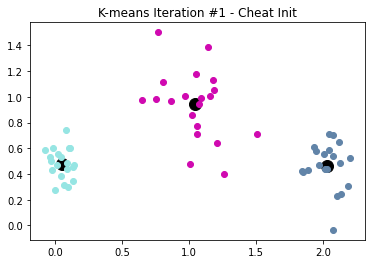
\includegraphics[scale=0.6]{2f-1.png}
\end{center}

\begin{center}
    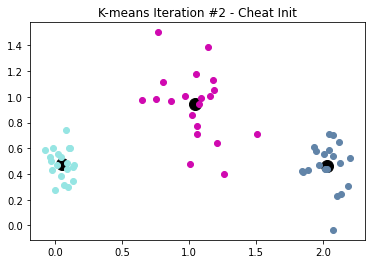
\includegraphics[scale=0.6]{2f-2.png}
\end{center}

Likewise, it was observed that when the centers were initialized by cheating, only one iteration was required for K-medoids. The algorithm ran for two iterations to confirm that the results of the first and second iteration were identical.

\begin{center}
    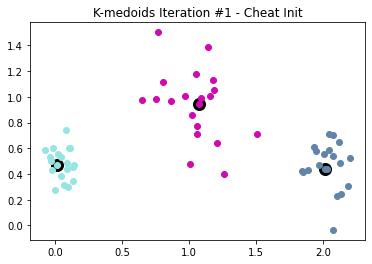
\includegraphics[scale=0.6]{2f-3.png}
\end{center}

\begin{center}
    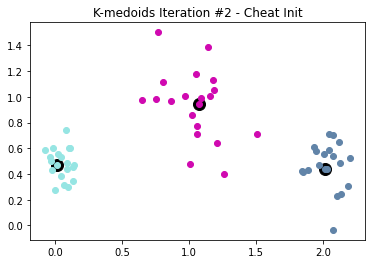
\includegraphics[scale=0.6]{2f-4.png}
\end{center}


\subsection{Clustering Faces}
\subsubsection{(a) Purity and time for kMeans and kMedoids}
\sol{} 
\begin{table}[H]
\centering
\begin{tabular}{l | cccccc}
            & average purity & min purity & max purity & average time & min time & max time\\ \hline
$k$-means   & 0.661250 & 0.525000 & 0.750000 & 0.217326 & 0.082916 & 0.449535\\
$k$-medoids & 0.603125 & 0.512500 & 0.668750 & 0.267117 & 0.201908 & 0.344556\\
\end{tabular}
\end{table}

According to the table provided, both k-means and k-medoids are incredibly close in terms of performance. However, k-means is ever-so-slightly superior since, on average, it has a marginally higher clustering performance score, a shorter runtime, and a higher maximum score. Although its maximum time is slightly higher than the maximum K-means time, the average score and time are likely the most reliable indicators of performance and runtime in this scenario.

\subsubsection{(b) Clustering score versus the number of components}
\sol x

\begin{center}
    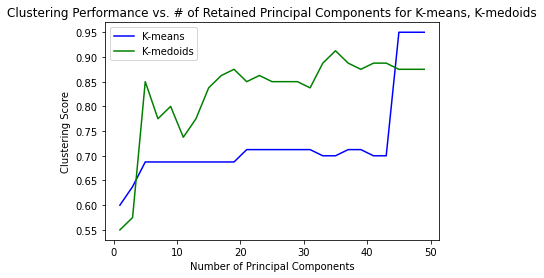
\includegraphics[scale=0.6]{3b.png}
\end{center}

As the number of principal components increases, both K-means and K-medoids exhibit improved performance, which is reasonable since it implies that more data is being retained, enabling the methods to better identify similarities and differences between image data points. Additionally, it is evident that K-medoids generally outperforms K-means, except in two instances: 1) when using only the first principal component, and 2) when using a large number of principal components (45 or more). At first, the performance difference between the two methods is minimal (for roughly l < 5), but as the value of l increases between 5 and 40, the performance gap between them quickly widens, and then the gap reduces again beyond 40, before K-means begins to perform better. In my opinion, K-medoids may have outperformed K-means because in facial recognition, it could be more advantageous for the cluster center to be an actual data point rather than an average.

\subsubsection{(c) Most similar and discriminative faces}
\sol x

I opted to choose all feasible combinations of pairs from the classes available to me, then selected 40 images from each class (same as in part (b)) and combined them to create a single image. Next, I used the K-medoids algorithm with two clusters (since we are comparing two images), along with a cheating initialization to ensure that the initialization would remain the same each time. I chose K-medoids instead of K-means, as my previous findings in part (b) suggested that K-medoids generally performed better. Then, I computed the clustering score for that specific pair of classes and, after calculating the clustering score for each pair, I determined the best and worst scores and identified the class pair they corresponded to.

\begin{center}
    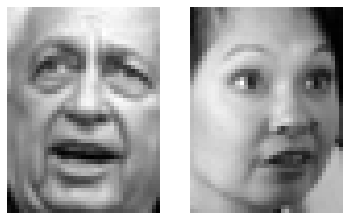
\includegraphics[scale=0.6]{3c-1.png}
\end{center}

Most different images: Best score of 0.9875, with images 0 and 6. These images clearly exhibit noticeable distinctions at first glance: the two individuals are facing opposite directions, and one is male while the other is female, resulting in dissimilar facial characteristics. The clustering score for this image set is the highest, as it can correctly allocate distinct features of each image to separate clusters.


\begin{center}
    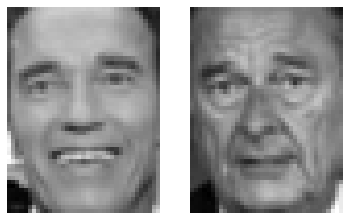
\includegraphics[scale=0.6]{3c-2.png}
\end{center}

Most similar images: Worst score of 0.5125, with images 1 and 8. In contrast to the previous image set, these two images appear very alike. They are both of men who are looking in the same direction, have similar hues and brightness, and even have comparable wrinkle patterns around their nose and mouth. As a result, it's understandable why this would lead to a low clustering score because K-medoids struggles to differentiate between the features of the two images, making it difficult to assign them to separate clusters.

\end{document}
